\chapter{Liikennevalot}

Lähdetään rakentamaan risteykseen ohjattuja liikennevaloja. Tässä osiossa aloita tyhjästä koekytkentälevystä.

\section{Ohjelmoitava valo}
\begin{minipage}{0.5\textwidth}
\begin{tcolorbox}[colback=lime!10,title=Tarvikkeet, colbacktitle=green!10,coltitle=black]
\begin{itemize}
    \item Punainen LED
    \item Vastus 220$\Omega$: 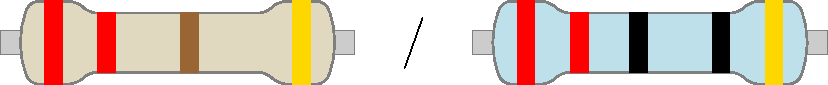
\includegraphics[width=0.5\textwidth]{kuvat/220.pdf}
    \item Hyppylankoja
    \item Arduino + koekytkentälevy
\end{itemize}
\end{tcolorbox}
\end{minipage}
\begin{minipage}{0.5\textwidth}
\begin{tcolorbox}[colback=blue!10,title=Piirin toiminta,colbacktitle=purple!90]
Ensimmäinen ohjelmoitava piiri. Kirjoitetaan koodi, joka sytyttää ja sammuttaa valon koodin mukaisesti.
\tcblower
\begin{center}
\begin{tikzpicture}
\ctikzset{american}
\draw (0,4) to [led,l=punainen,fill=red] (0,2);
\draw (0,2) to[R,a=$220\Omega$] (0,0);
\draw (0,0) -- (0,-0.5) node[ground]{}; 
\draw (-1,4) node[left] {7} to[short,o-] (0,4);
\end{tikzpicture}
\end{center}
\end{tcolorbox}
\end{minipage}

\begin{tcolorbox}[colback=red!10,colbacktitle=red,title=HUOM!]
Aina kun rakennat tai muutat piiriä, pidä Arduino irrotettuna tietokoneesta! 
\tcblower
Muista tarkistaa miten päin LEDit kytketään! Tämä löytyy esimerkiksi sivulta \pageref{box:led}.
\end{tcolorbox}

Aiemmin käytimme painonappia valon ohjaamiseen, ja painamalla nappia saimme valon syttymään. Nyt tehdään kytkentä, jonka avulla saadaan valo automaattisesti sammumaan ja syttymään. 


Kytketään ensin punainen LED ja vastus koekytkentälevylle. Ja kytketään myös $-$ maahan.

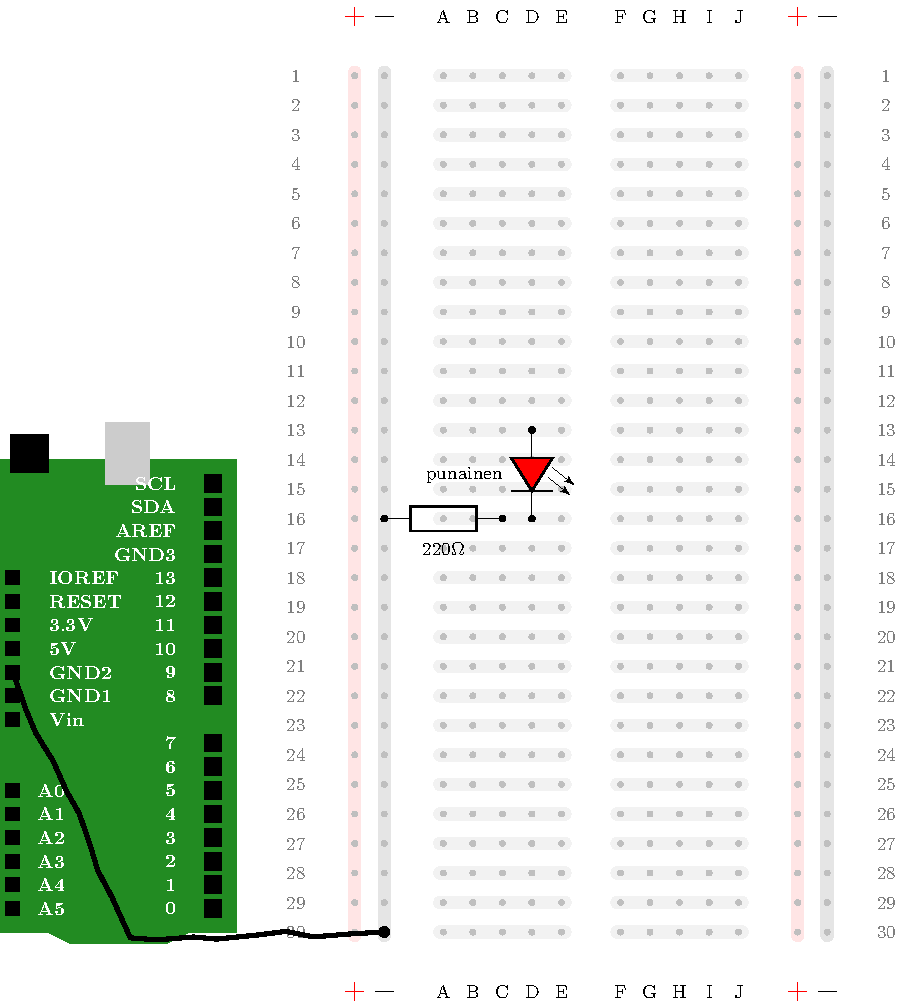
\includegraphics[width=0.95\textwidth]{kuvat/kuva7.pdf}

Aiemmassa kytkennässä rivi 13 kytkettiin suoraan vakiojännitelähteeseen, 5V, mutta nyt koska haluamme ohjelmoida, kytketään rivi 13 käyttämältämme puolelta ohjelmoitavaan pinniin 7 Arduinossa.

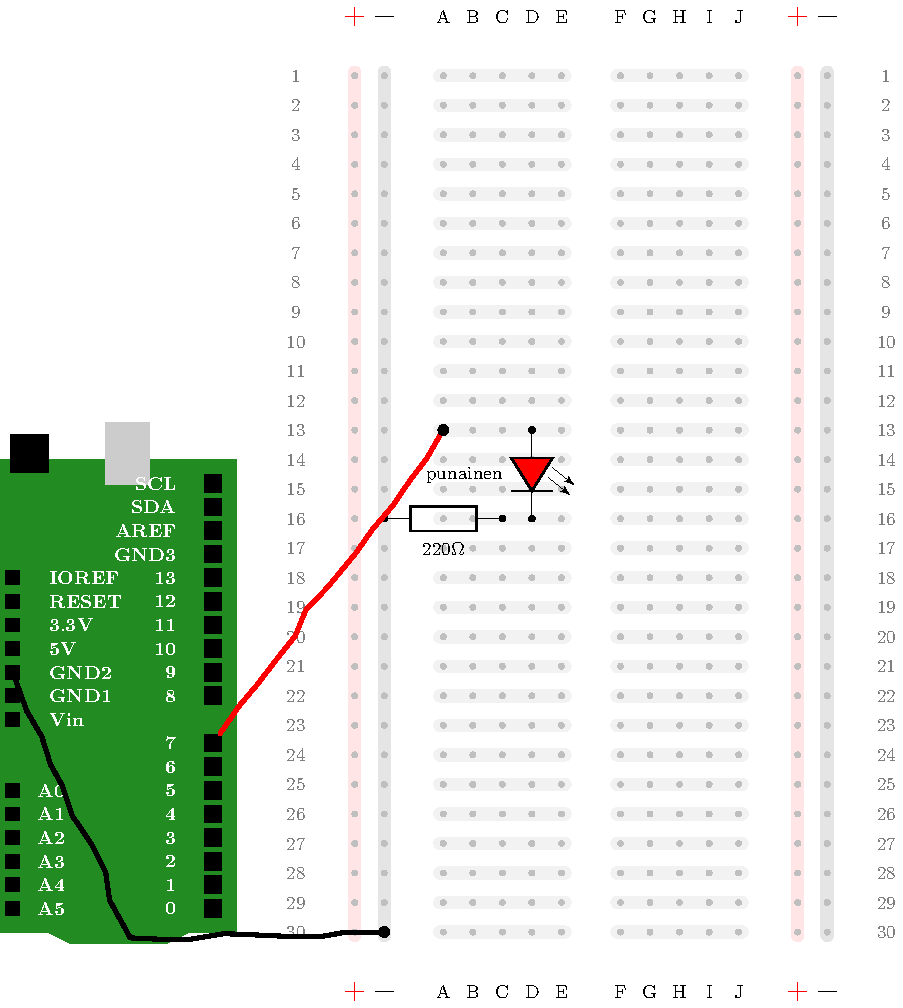
\includegraphics[width=0.8\textwidth]{kuvat/kuva8.pdf}

Avataan nyt Arduino-sovellus, ja kopioidaan alla oleva koodi sinne.


\begin{lstlisting}[numbers=none]
void setup() {
pinMode(7, OUTPUT); // Punainen LED on pinnissa 7
}

void loop() {
digitalWrite(7, HIGH); // Laitetaan valo paalle
delay(1000); // Odotetaan
digitalWrite(7, LOW); // Laitetaan valo pois paalta
delay(1000); // Odotetaan
}
\end{lstlisting}


Käydään vielä koodi lävitse: 

Rivit 1-3 ovat alustamista (asetukset) varten. Rivillä 3 kerrotaan mitä haluamme tehdä pinnillä 7: haluamme ohjata tällä valoa, joten tyyppi on OUTPUT.

Rivit 5-10 ovat miten haluamme ohjata valoa. Kirjoittamalla rivin 6 koodin, asetamme pinnin 7 arvoksi HIGH, eli korkea, eli 5V, ja kuten tiedämme aiemmasta piiristämme, tällöin valo palaa. Sitten seuraavalla rivillä odotamme 1000ms (millisekuntia, eli yhden sekunnin), kunnes teemme rivin 8 operaation: muutamme pinnin 7 arvoksi LOW, eli matala, eli 0V, ja sammutamme valon. Tämän jälkeen odotamme taas yhden sekunnin. Koska koodi on kirjoitettu silmukkaan (loop), toistamme tätä, kunnes kytkemme piirin irti jännitelähteestä.

Nyt voit ladata Arduinolle koodin ja katsoa mitä tapahtuu! Voit myös testata odotusajan muuttamista muuttamalla lukuja 1000 koodissa. Muista, että kyseessä on millisekunnit, joten jos haluat, että valo on päällä 3s ja pois päältä 2s, ensimmäinen 1000 pitää muuttaa luvuksi 3000 ja toinen luvuksi 2000. 

\begin{tcolorbox}[colback=white,title=Vinkkejä Arduinolla koodaamiseen!,colbacktitle=purple!90]
Seuraavassa esitellään Arduinolla koodaamiseen liittyviä vinkkejä. 
\begin{lstlisting}
// Kaksi kauttaviivaa aloittaa kommentin. Tata ei siis lueta koodissa vaan on tiedoksi koodin lukijalle

pinMode(luku, tyyppi) // Talla voit saataa pinnien 0-13 tekoa laittamalla sanan luku tilalle luvun jolta rivilta haluat komentaa
// Tyypin tilalle voit kirjoittaa joko OUTPUT eli Arduino lahettaa signaalia
// tai INPUT jolloin Arduino vastaanottaa signaalin

digitalWrite(luku, arvo) // Talla voit muuttaa pinniin luku kirjoitettua arvoa
// arvo HIGH vastaa 5V jannitetta
// arvo LOW vastaa 0V jannitetta

delay(luku) // Odottaa luvun verran millisekunteja
\end{lstlisting}
\end{tcolorbox}

\section{Ohjelmoitava liikennevalo}

\begin{tcolorbox}[colback=lime!10,title=Tarvikkeet, colbacktitle=green!10,coltitle=black]
\begin{itemize}
    \item Edellisen kohdan piiri rakennettuna
    \item Keltainen LED ja vihreä LED
    \item 2 kpl 220$\Omega$: 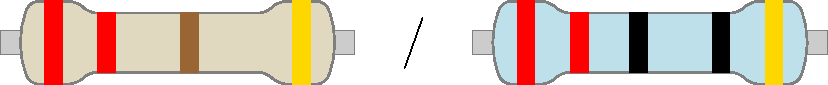
\includegraphics[width=0.5\textwidth]{kuvat/220.pdf}
    \item Hyppylankoja
\end{itemize}
\end{tcolorbox}


\begin{tcolorbox}[colback=blue!10,title=Piirin toiminta,colbacktitle=purple!90]
Kirjoitetaan koodi, jonka avulla saadaan liikennevalot toimimaan.
\tcblower
\begin{center}
\begin{tikzpicture}[]
\ctikzset{american}
\draw (0,4) to [led,l=punainen,fill=red] (0,2);
\draw (0,2) to[R,a=$220\Omega$] (0,0);
\draw (0,0) -- (0,-0.5) node[ground]{}; 
\draw (-1,4) node[left] {7} to[short,o-] (0,4);

\draw (3,4) to [led,l=keltainen,fill=yellow] (3,2);
\draw (3,2) to[R,a=$220\Omega$] (3,0);
\draw (3,0) -- (3,-0.5) node[ground]{}; 
\draw (2,4) node[left] {4} to[short,o-] (3,4);

\draw (6,4) to [led,l=vihreä,fill=green] (6,2);
\draw (6,2) to[R,a=$220\Omega$] (6,0);
\draw (6,0) -- (6,-0.5) node[ground]{}; 
\draw (5,4) node[left] {3} to[short,o-] (6,4);

\end{tikzpicture}
\end{center}
\end{tcolorbox}


\begin{tcolorbox}[colback=red!10,colbacktitle=red,title=HUOM!]
Aina kun rakennat tai muutat piiriä, pidä Arduino irrotettuna tietokoneesta! 
\end{tcolorbox}

Lisätään ensin keltainen ja vihreä LED ja niiden kanssa sarjassa olevat vastukset ja kytketään keltainen LED pinniin 4 ja vihreä LED pinniin 3. Huomaa, että hyppylankojen värillä ei ole väliä. Selvyyden vuoksi kuvassa on käytetty samaa väriä kuin mihin LEDiin ollaan yhdistämässä.

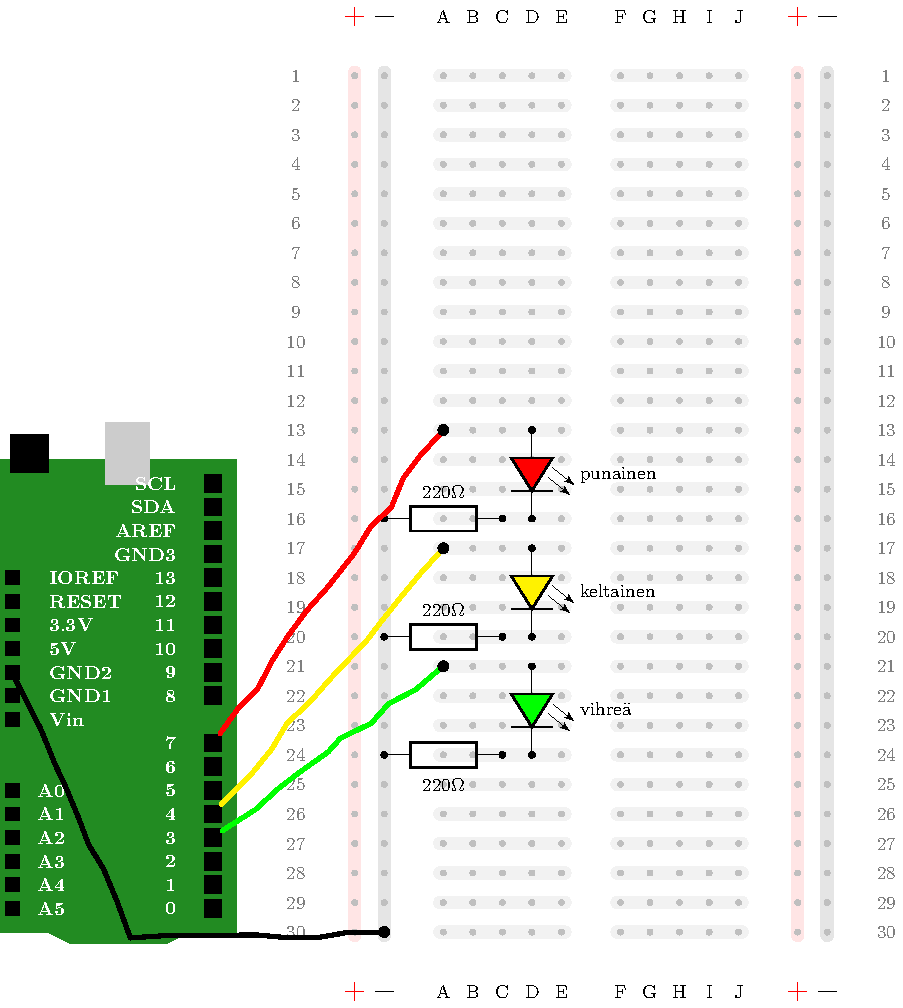
\includegraphics[width=0.95\textwidth]{kuvat/kuva9.pdf}

Nyt lisätään keltaiselle ja vihreällä LEDille (vastaavasti kuin punaisella LEDillä jo on), tieto siitä mitä pinneillä 4 ja 3 halutaan tehdä.
\clearpage
\begin{lstlisting}[numbers=none] 
void setup() {
pinMode(7, OUTPUT); // Punainen LED on pinnissa 7
pinMode(4, OUTPUT); // Keltainen LED on pinnissa 4
pinMode(3, OUTPUT); // Vihrea LED on pinnissa 2
}

void loop() {
digitalWrite(7, HIGH); // Laitetaan punainen valo paalle
digitalWrite(4, HIGH); // Laitetaan keltainen valo paalle
digitalWrite(3, HIGH); // Laitetaan vihrea valo paalle
delay(1000); // Odotetaan
digitalWrite(7, LOW); // Laitetaan punainen valo pois paalta
digitalWrite(4, LOW); // Laitetaan keltainen valo pois paalta
digitalWrite(3, LOW); // Laitetaan vihrea valo pois paalta
delay(1000); // Odotetaan
}
\end{lstlisting}

Nyt yllä oleva koodi vilkuttaa kaikkea kolmea valoa yhtä aikaa. Vaihda rivien järjestystä, ja lisää tarvittaessa odotuskomentoja tai päälle/pois komentoja, jotta saat valot ohjelmoitua. 

\begin{tcolorbox}[colback=yellow!10, title={Koodaa!},colbacktitle=orange]
Miten muutat koodia, jotta saat liikennevalot toimimaan kuten oikeat valot toimivat? 
\begin{solution}
\begin{lstlisting}
void setup() {
pinMode(7, OUTPUT); // Punainen LED on pinnissa 7
pinMode(4, OUTPUT); // Keltainen LED on pinnissa 4
pinMode(3, OUTPUT); // Vihrea LED on pinnissa 2
}

void loop() {
digitalWrite(7, HIGH); // Laitetaan punainen valo paalle
delay(1000); // Odotetaan
digitalWrite(4, HIGH); // Laitetaan keltainen valo paalle
delay(1000); // Odotetaan
digitalWrite(7, LOW); // Laitetaan punainen valo pois paalta
digitalWrite(4, LOW); // Laitetaan keltainen valo pois paalta
digitalWrite(3, HIGH); // Laitetaan vihrea valo paalle
delay(1000); // Odotetaan
digitalWrite(3, LOW); // Laitetaan vihrea valo pois paalta
digitalWrite(4, HIGH); // Laitetaan keltainen valo paalle
delay(1000);
digitalWrite(4, LOW); // Laitetaan keltainen valo pois paalta
digitalWrite(7, HIGH); // Laitetaan punainen valo paalle
delay(1000); // Odotetaan
}

\end{lstlisting}
Kyseessä on esimerkkikoodi, ja tämän jälkeen voidaan puhua siitä, kauanko kukin valo palaa ja tarvitseeko viimeisenä olla punainen valo päälle vai ei.
\end{solution}
\end{tcolorbox}

%%%%%%%%%%%%%%%%%%%%%%%%%%%%%%%%%5
\clearpage
\section{Painonapin lisääminen}
\begin{tcolorbox}[colback=lime!10,title=Tarvikkeet, colbacktitle=green!10,coltitle=black]
\begin{itemize}
    \item Edellisen kohdan piiri rakennettuna
    \item Painonappi
    \item Vastus 220$\Omega$: 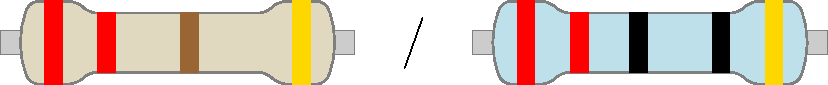
\includegraphics[width=0.5\textwidth]{kuvat/220.pdf}
    \item Hyppylankoja
\end{itemize}
\end{tcolorbox}


\begin{tcolorbox}[colback=blue!10,title=Piirin toiminta,colbacktitle=purple!90]
Lisätään painonappi, jota painamalla saadaan liikennevalojen toiminta muuttumaan.
\end{tcolorbox}

\begin{tcolorbox}[colback=red!10,colbacktitle=red,title=HUOM!]
Aina kun rakennat tai muutat piiriä, pidä Arduino irrotettuna tietokoneesta! 
\end{tcolorbox}

Käytimme jo aiemmin painonappia manuaalisesti valon ohjaamiseen, mutta lisätään tämä nyt koodimme. Lisää aiempaan kytkentääsi painonappi sekä vastus ja kolme hyppylankaa (kuvassa punainen ja kaksi sinistä).

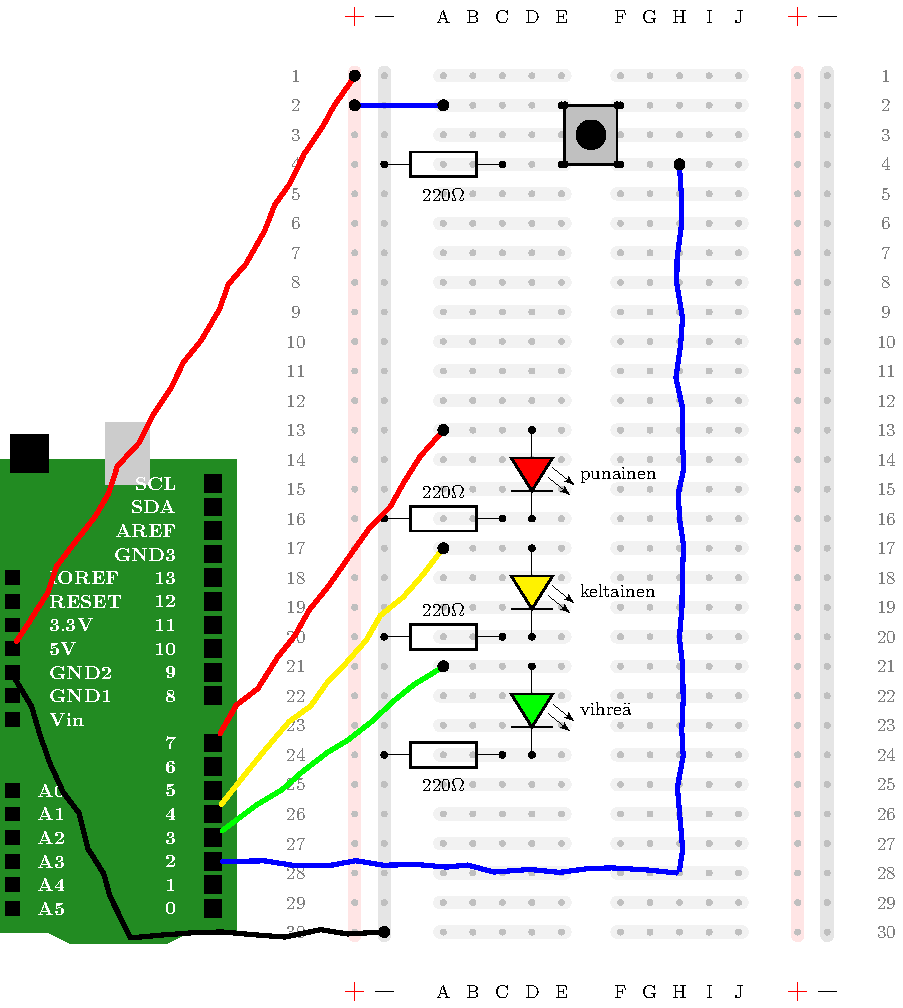
\includegraphics[width=0.9\textwidth]{kuvat/kuva10.pdf}

% \begin{tikzpicture}[scale=0.5]
% \pic[scale=0.2] at (0,0) {myarduino};
% \BREADBOARD(20,30){30};
% \draw (C16) to[R,a=$220\Omega$,*-*] (lg16);
% \draw (D13) to[led,l=punainen,*-*,fill=red] (D16);
% \draw[black,wire] (ArGND2) -- ++(4,-9) to[short,-*] (lg30);
% \draw[wire,red] (A13) to[short,*-*] (Ar7);

% \draw (C20) to[R,a=$220\Omega$,*-*] (lg20);
% \draw (D17) to[led,l=keltainen,*-*,fill=yellow] (D20);
% \draw[wire,yellow] (A17) to[short,*-*] (Ar4);

% \draw (C24) to[R=$220\Omega$,*-*] (lg24);
% \draw (D21) to[led,l=vihreä,*-*,fill=green] (D24);
% \draw[wire,green] (A21) to[short,*-*] (Ar3);

% % Painonappi
% \draw[thick,fill=hopea] (E2.east) rectangle (F4.west) coordinate[pos=0.5] (Y);
% \draw[fill=black] (Y) circle (0.5);
% \draw (E2.east) to[short,*-*] (E2);
% \draw (E4.east) to[short,*-*] (E4);
% \draw (F4.west) to[short,*-*] (F4);
% \draw (F2.west) to[short,*-*] (F2);
% % Vastus
% \draw (C4) to[R=$220\Omega$,*-*] (lg4);
% % Kayttojannite
% \draw[red,wire] (l-1) to[short,*-*] (Ar5V);
% % Painonapin kytkentä
% \draw[blue,wire] (l-2) to[short,*-*] (A2);
% \draw[blue,wire] (H4) to[short,*-]  (H28) to[short,-*] (Ar2);
% \end{tikzpicture}

\clearpage
Nyt muokataan koodia ottamaan huomioon painonappi. Tämä esimerkkikoodi sytyttää kaikki valot kun nappia painetaan ja ne sammuvat kun nappia ei paineta.

\begin{lstlisting}[numbers=none]
void setup() {
pinMode(7, OUTPUT); // Punainen LED on pinnissa 7
pinMode(4, OUTPUT); // Keltainen LED on pinnissa 4
pinMode(3, OUTPUT); // Vihrea LED on pinnissa 2
pinMode(2, INPUT); // Lisataan painonappi tuloksi
}

void loop() {
  bool buttonState = digitalRead(2); // Luetaan painonapin tila

  // Tarkastetaan onko nappi painettu
  if (buttonState == HIGH){
    // Jos on laitetaan LEDit paalle
    digitalWrite(7, HIGH); // Laitetaan punainen valo paalle
    digitalWrite(4, HIGH); // Laitetaan keltainen valo paalle
    digitalWrite(3, HIGH); // Laitetaan vihrea valo paalle
  } else {
    // Jos ei, niin laitetaan LEDit pois paalta
    digitalWrite(7, LOW); // Laitetaan punainen valo pois paalta
    digitalWrite(4, LOW); // Laitetaan keltainen valo pois paalta
    digitalWrite(3, LOW); // Laitetaan vihrea valo pois paalta
  }
}
\end{lstlisting}

\begin{tcolorbox}[colback=white,title=Vinkkejä Arduinolla koodaamiseen!,colbacktitle=purple!90]
\begin{lstlisting}
muuttuja = digitalRead(luku); // Lukee pinnin luku arvon ja tallentaa sen muuttujaan muuttuja
// Huomaa etta muuttujalla pitaa olla annettuna tyyppi
// Esimerkiksi bool:
bool muuttuja = digitalRead(luku); 
// bool voi olla joko HIGH tai LOW sen mukaan mita tassa tapauksessa luettiin piirista
// bool on kateva tilanteissa joissa arvo on joko HIGH tai LOW

// Ehtorakenne
// Tarkastetaan muuttujan arvo.
if (muuttuja == HIGH) {
   // jos muuttujan arvo on HIGH tehdaan koodi tassa valissa
} else {
   // muuten (eli kun LOW) tehdaan mita tassa kirjoitetaan
}
\end{lstlisting}
\end{tcolorbox}

\begin{tcolorbox}[title=Haaste!,colback=teal!10,colbacktitle=teal!90]
Miten muutat koodia, jotta kun nappia painetaan, vilkkuu vain keltainen valo ja kun nappia ei paineta, liikennevalot toimivat normaalisti? 
\end{tcolorbox}

\begin{tcolorbox}[colback=yellow!10, title={Koodaa!},colbacktitle=orange,breakable]
\begin{solution}
\begin{lstlisting}
void setup() {
pinMode(7, OUTPUT); // Punainen LED on pinnissa 7
pinMode(4, OUTPUT); // Keltainen LED on pinnissa 4
pinMode(3, OUTPUT); // Vihrea LED on pinnissa 2
pinMode(2, INPUT); // Lisataan painonappi tuloksi
}

void loop() {
  bool buttonState = digitalRead(2); // Luetaan painonapin tila
  // Tarkastetaan onko nappi painettu
  if (buttonState == HIGH){
    // Jos on laitetaan LEDit paalle
    digitalWrite(4, HIGH); // Laitetaan keltainen valo paalle
    digitalWrite(7, LOW); // Sammutetaan varmuuden vuoksi punainen valo
    digitalWrite(3, LOW); // Sammutetaan varmuuden vuoksi vihrea valo
    delay(1000); // Odotetaan
    digitalWrite(4,LOW); // Laitetaan keltainen valo pois paalta
    delay(1000);
  } else {
    digitalWrite(7, HIGH); // Laitetaan punainen valo paalle
    delay(1000); // Odotetaan
    digitalWrite(4, HIGH); // Laitetaan keltainen valo paalle
    delay(1000); // Odotetaan
    digitalWrite(7, LOW); // Laitetaan punainen valo pois paalta
    digitalWrite(4, LOW); // Laitetaan keltainen valo pois paalta
    digitalWrite(3, HIGH); // Laitetaan vihrea valo paalle
    delay(1000); // Odotetaan
    digitalWrite(3, LOW); // Laitetaan vihrea valo pois paalta
    digitalWrite(4, HIGH); // Laitetaan keltainen valo paalle
    delay(1000);
    digitalWrite(4, LOW); // Laitetaan keltainen valo pois paalta
    digitalWrite(7, HIGH); // Laitetaan punainen valo paalle
    delay(1000); // Odotetaan
  }
}
\end{lstlisting}
Nyt huomionarvoista on se, koska piiri reagoi napinpainallukseen? Yllä olevalla koodilla reagointi tapahtuu vasta kun valo on vaihdettu punaiseksi ja valot käynnistyvät taas punaisesta, kun napista päästetään irti.
\end{solution}
\end{tcolorbox}

\begin{tcolorbox}[title=Haaste!,colback=teal!10,colbacktitle=teal!90]
Laita nappi toimimaan valokatkaisijan tavoin. Kun nappia painetaan kerran, alkaa ohjelma vilkuttamaan keltaista valoa ja jos nappia painetaan uudelleen, liikennevalot toimivat taas.
\end{tcolorbox}

\begin{tcolorbox}[colback=white,title=Vinkkejä Arduinolla koodaamiseen!,colbacktitle=purple!90]
\begin{lstlisting}
bool ledStatus = true; // Luodaan muuttuja, jonka arvo on totta

ledStatus = !ledStatus; // Muuttaa muuttujan ledStatus arvoksi arvon epatosi (jos arvo oli tosi) tai tosi (jos arvo oli epatosi)
\end{lstlisting}
\end{tcolorbox}

\begin{tcolorbox}[colback=yellow!10, title={Koodaa!},colbacktitle=orange,breakable]
\begin{solution}
\begin{lstlisting}
// Alustetaan muuttuja
bool ledStatus = true;

void setup() {
pinMode(7, OUTPUT); // Punainen LED on pinnissa 7
pinMode(4, OUTPUT); // Keltainen LED on pinnissa 4
pinMode(3, OUTPUT); // Vihrea LED on pinnissa 2
pinMode(2, INPUT); // Lisataan painonappi tuloksi
}

void loop() {
  bool buttonState = digitalRead(2); // Luetaan painonapin tila
  
  if (buttonstate == HIGH) {
    ledStatus = !ledStatus
  }
  
  // Tarkastetaan mita tehdaan
  if (ledStatus == HIGH){
    // Jos on laitetaan LEDit paalle
    digitalWrite(4, HIGH); // Laitetaan keltainen valo paalle
    digitalWrite(7, LOW); // Sammutetaan varmuuden vuoksi punainen valo
    digitalWrite(3, LOW); // Sammutetaan varmuuden vuoksi vihrea valo
    delay(1000); // Odotetaan
    digitalWrite(4,LOW); // Laitetaan keltainen valo pois paalta
    delay(1000);
  } else {
    digitalWrite(7, HIGH); // Laitetaan punainen valo paalle
    delay(1000); // Odotetaan
    digitalWrite(4, HIGH); // Laitetaan keltainen valo paalle
    delay(1000); // Odotetaan
    digitalWrite(7, LOW); // Laitetaan punainen valo pois paalta
    digitalWrite(4, LOW); // Laitetaan keltainen valo pois paalta
    digitalWrite(3, HIGH); // Laitetaan vihrea valo paalle
    delay(1000); // Odotetaan
    digitalWrite(3, LOW); // Laitetaan vihrea valo pois paalta
    digitalWrite(4, HIGH); // Laitetaan keltainen valo paalle
    delay(1000);
    digitalWrite(4, LOW); // Laitetaan keltainen valo pois paalta
    digitalWrite(7, HIGH); // Laitetaan punainen valo paalle
    delay(1000); // Odotetaan
  }
}
\end{lstlisting}

Nyt huomattavaa on se, että napin painallus pitää ajoittaa oikein, sillä väärässä vaiheessa napin painallusta ei huomata, eli nappia on painettava pitkään, jotta muutos välittyy koodille.
\end{solution}
\end{tcolorbox}

\begin{tcolorbox}[title=Haaste!,colback=teal!10,colbacktitle=teal!90]
Muuta koodin toimintaa niin, että edellinen koodi reagoi heti kun nappia painetaan.
\end{tcolorbox}

\begin{tcolorbox}[colback=white,title=Vinkkejä Arduinolla koodaamiseen!,colbacktitle=purple!90]
\begin{lstlisting}
// Seuraava rivi lisataan setup() funktioon
attachInterrupt(digitalPinToInterrupt(luku), keskeytys, FALLING);
// attachInterrupt on komento jolla luodaan keskeytys
// digitalPinToInterrupt(luku) kertoo mista pinnista saadaan painallus
// keskeytys on aliohjelmanne nimi, johon siirrytaan
// FALLING on parametri joka tarkoittaa kun nappia painetaan alas
// Vaihtoehtona ovat myos
// LOW kun pinnin luku jannite on 0V
// CHANGE kun pinnin luku jannite muuttuu
// RISING kun pinnin tila muuttuu nollasta viiteen volttiin
// FALLING kun pinnin tila muuttuu viidesta voltista nollaan

// Maaritetaan uusi funktio olemassa olevien peraan
void keskeytys() {
  // Mita funktio tekee?
  // Esimerkiksi vaihtaa muuttujan ledState arvo:
  ledState = !ledState;
}
// Talloin ohjelman alussa pitaa olla maaritys
volative bool ledState = false;
// volative tarkoittaa, etta muuttujan arvo tarkastetaan aina sita kaytettaessa
// muuttujan ledState arvo voi siis muuttua milloin vain ohjelman aikana
\end{lstlisting}
\end{tcolorbox}

\begin{tcolorbox}[colback=yellow!10, title={Koodaa!},colbacktitle=orange,breakable]
\begin{solution}
\begin{lstlisting}
// Alustetaan muuttuja
volatile bool ledStatus = false;

void setup() {
pinMode(7, OUTPUT); // Punainen LED on pinnissa 7
pinMode(4, OUTPUT); // Keltainen LED on pinnissa 4
pinMode(3, OUTPUT); // Vihrea LED on pinnissa 2
pinMode(2, INPUT); // Lisataan painonappi tuloksi
attachInterrupt(digitalPinToInterrupt(2), keskeytys, FALLING);
}

void loop() {
  // Tarkastetaan onko nappi painettu
  if (ledStatus == HIGH){
    // Jos on laitetaan LEDit paalle
    digitalWrite(4, HIGH); // Laitetaan keltainen valo paalle
    digitalWrite(7, LOW); // Sammutetaan varmuuden vuoksi punainen valo
    digitalWrite(3, LOW); // Sammutetaan varmuuden vuoksi vihrea valo
    delay(1000); // Odotetaan
    digitalWrite(4,LOW); // Laitetaan keltainen valo pois paalta
    delay(1000);
  } else {
    digitalWrite(7, HIGH); // Laitetaan punainen valo paalle
    delay(1000); // Odotetaan
    digitalWrite(4, HIGH); // Laitetaan keltainen valo paalle
    delay(1000); // Odotetaan
    digitalWrite(7, LOW); // Laitetaan punainen valo pois paalta
    digitalWrite(4, LOW); // Laitetaan keltainen valo pois paalta
    digitalWrite(3, HIGH); // Laitetaan vihrea valo paalle
    delay(1000); // Odotetaan
    digitalWrite(3, LOW); // Laitetaan vihrea valo pois paalta
    digitalWrite(4, HIGH); // Laitetaan keltainen valo paalle
    delay(1000);
    digitalWrite(4, LOW); // Laitetaan keltainen valo pois paalta
    digitalWrite(7, HIGH); // Laitetaan punainen valo paalle
    delay(1000); // Odotetaan
  }
}

void keskeytys() {
  ledStatus = !ledStatus;
}
\end{lstlisting}
Lisäksi voi miettiä esimerkiksi miten jalankulkijan painonapin saisi mukaan. Huomaa, että tämän työn kanssa on tärkeää painaa painonappia hyvin, Arduino ei aina kunnolla huomaa tai huomaa liian monta painallusta putkeen yhden sijasta. Tätä voi kiertää koodaamalla esimerkiksi ajastimen painallusten välisen ajan havainnointiin, mutta tämä on jätetty ohjeesta pois.
\end{solution}
\end{tcolorbox}

\section{Suunnittelu omat liikennevalot risteykseen}
Nyt kun ohjelmointia on kokeiltu monelta eri kannalta, voit suunnitella kokonaisen risteyksen liikennevalot. Piirrä alle risteyksesi. Lisäksi on tilaa piirtää kuva koekytkentälevystäsi, jotta näet miten olet piirin kytkenyt. Sitä seuraavalla sivulla on tilaa suunnitella koodiasi.

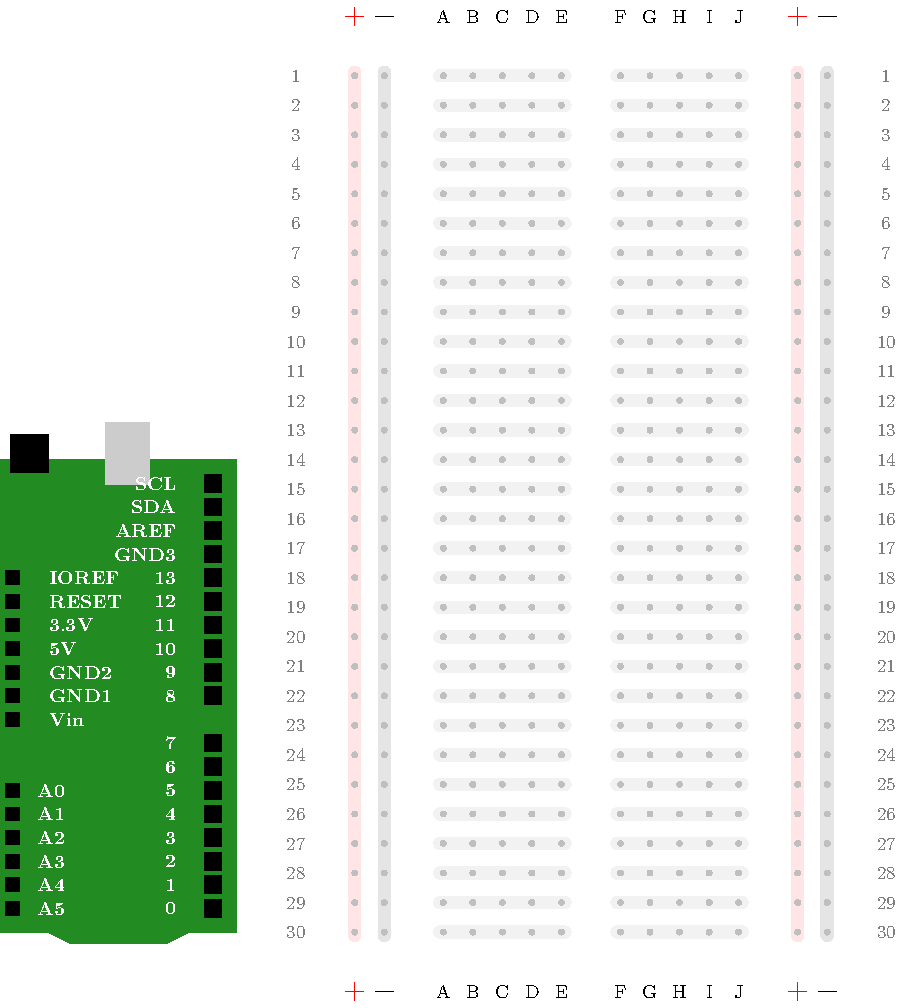
\includegraphics[width=0.9\textwidth]{kuvat/kuva11.pdf}

\begin{tcolorbox}[colback=yellow!10, title={Koodaa!},colbacktitle=orange,breakable]
\begin{solution}
\vspace{18cm}
Tähän tehtävään ei ole malliratkaisua.
\end{solution}
\end{tcolorbox}